\documentclass[11pt,fleqn]{article}

\setlength {\topmargin} {-.15in}
\setlength {\textheight} {8.6in}

\usepackage{amsmath}
\usepackage{amssymb}
\usepackage{amsthm}
\usepackage{color}
\usepackage[utf8]{inputenc}
\usepackage{listings}
\usepackage{fullpage}
\usepackage{fancyvrb}
\usepackage{graphicx}

\graphicspath{ {./images/} }


\renewcommand{\labelenumii}{\theenumii.}

\newcommand{\mname}[1]{\mbox{\sf #1}}
\newcommand{\pnote}[1]{{\langle \text{#1} \rangle}}
\newcommand\todo[1]{\textcolor{red}{[TODO: #1]}}


\begin{document}

\begin{center}

  {\large \textbf{COMPSCI/SFWRENG 2C03}}\\[2mm]
  {\large \textbf{Data Structures and Algorithms}}\\[2mm]
  {\large \textbf{Ryszard Janicki}}\\[2mm]
  {\large \textbf{McMaster University}}\\[6mm]
  {\huge \textbf{Assignment 3}}\\[6mm]
  {\large \textbf{Name: Hishmat Salehi}}\\[2mm]
  {\large \textbf{MacId: Salehh6}}\\[2mm]
  {\large \textbf{Student number: 400172262}}\\[2mm]


\end{center}

\medskip

\begin{enumerate}

%Q1
	\item 	
		\begin{enumerate}
			\item 
0: 5 $\rightarrow$ 2 $\rightarrow$ 6 \\
1: 4 $\rightarrow$ 8 $\rightarrow$ 11 \\
2: 5 $\rightarrow$ 6 $\rightarrow$ 0 $\rightarrow$ 3 \\
3: 10 $\rightarrow$ 6 $\rightarrow$ 2 \\
4: 1 $\rightarrow$ 8 \\
5: 0 $\rightarrow$ 10 $\rightarrow$ 2 \\
6: 2 $\rightarrow$ 3 $\rightarrow$ 0 \\
7: 8 $\rightarrow$ 11 \\
8: 1 $\rightarrow$ 11 $\rightarrow$ 7 $\rightarrow$ 4 \\
9: \\
10: 5 $\rightarrow$ 3 \\
11: 8 $\rightarrow$ 7 $\rightarrow$ 1
			\item Adjacency Matrix:

\begin{verbatim}
0, 0, 1, 0, 0, 1, 1, 0, 0, 0, 0, 0, 
0, 0, 0, 0, 1, 0, 0, 0, 1, 0, 0, 1, 
1, 0, 0, 1, 0, 1, 1, 0, 0, 0, 0, 0, 
0, 0, 1, 0, 0, 0, 1, 0, 0, 0, 1, 0, 
0, 1, 0, 0, 0, 0, 0, 0, 1, 0, 0, 0, 
1, 0, 1, 0, 0, 0, 0, 0, 0, 0, 1, 0, 
1, 0, 1, 1, 0, 0, 0, 0, 0, 0, 0, 0, 
0, 0, 0, 0, 0, 0, 0, 0, 1, 0, 0, 1, 
0, 1, 0, 0, 1, 0, 0, 1, 0, 0, 0, 1, 
0, 0, 0, 0, 0, 0, 0, 0, 0, 0, 0, 0, 
0, 0, 0, 1, 0, 1, 0, 0, 0, 0, 0, 0, 
0, 1, 0, 0, 0, 0, 0, 1, 1, 0, 0, 0, 
\end{verbatim}
		\end{enumerate}

\newpage

%Q2
	\item $~$\\
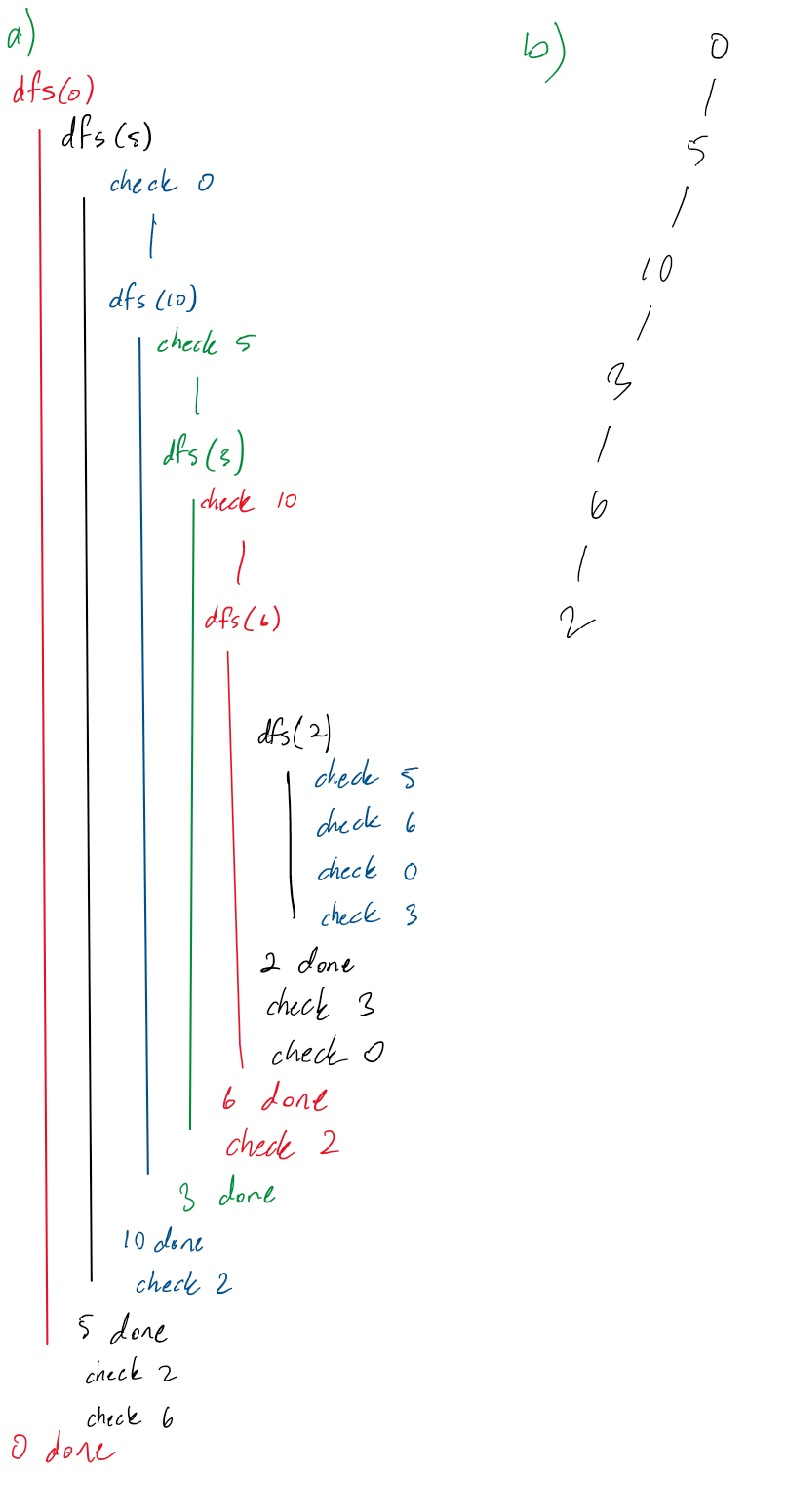
\includegraphics[scale=0.75]{Q2}

\newpage

%Q3
	\item $~$\\
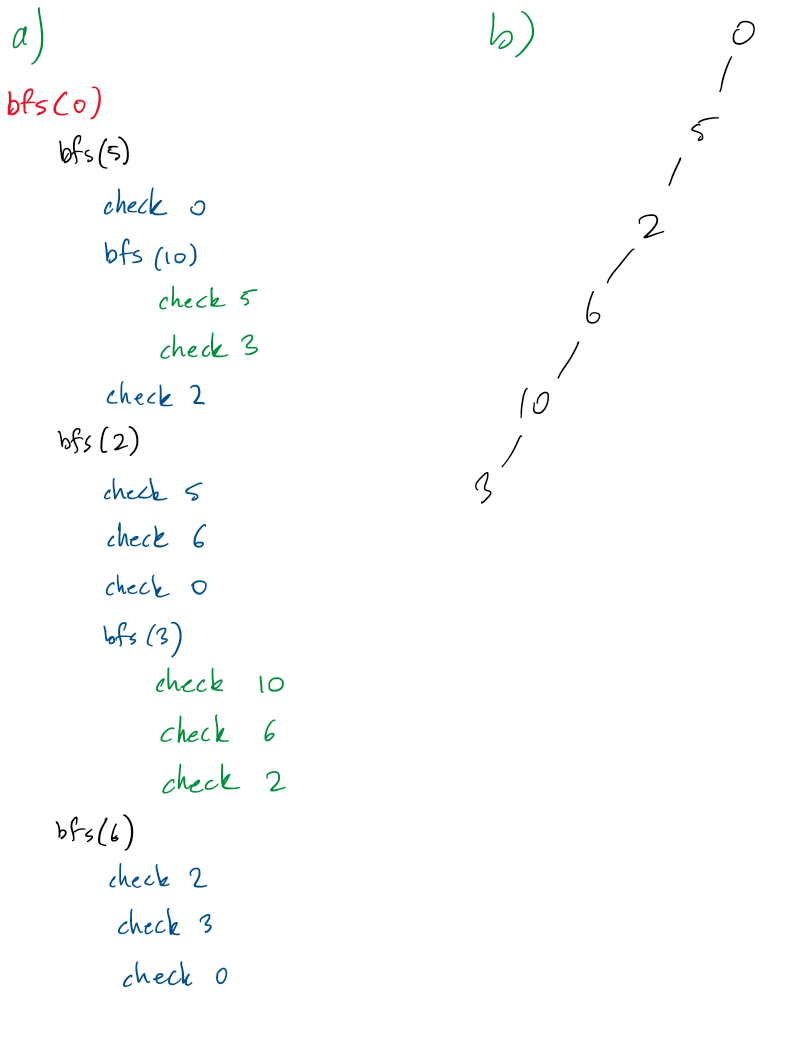
\includegraphics[scale=0.75]{Q3}

%Q4
	\item Consider by contradiction that the edge of maximum weight in the cycle C, edge e, belongs to the MST of the graph.
Since MSTs do not contain cycles there is at least one edge in C that is not in the MST. Let's call one of these edges f.
Now add f to the MST. There is now a cycle in the MST. Since e has the maximum weight in the cycle C and all edge weights are distinct, it means that weight(f) < weight(e). 
Removing the edge e after having added the edge f would generate a new MST' with total weight less than the total weight in MST, contradicting its minimality.

\newpage

%Q5
	\item 
		\begin{enumerate}
			\item
0: 6 $\rightarrow$ 5 \\
1: \\
2: 0 $\rightarrow$ 3 \\
3: 10 $\rightarrow$ 6 \\
4: 1 \\
5: 10 $\rightarrow$ 2 \\
6: 2 \\
7: 8 $\rightarrow$ 11 \\
8: 1 $\rightarrow$ 4 \\
9: \\
10: 3 \\
11: 8
			\item Adjacency Matrix:
\begin{verbatim}
0, 0, 0, 0, 0, 1, 1, 0, 0, 0, 0, 0, 
0, 0, 0, 0, 0, 0, 0, 0, 0, 0, 0, 0, 
1, 0, 0, 1, 0, 0, 0, 0, 0, 0, 0, 0, 
0, 0, 0, 0, 0, 0, 1, 0, 0, 0, 1, 0, 
0, 1, 0, 0, 0, 0, 0, 0, 0, 0, 0, 0, 
0, 0, 1, 0, 0, 0, 0, 0, 0, 0, 1, 0, 
0, 0, 1, 0, 0, 0, 0, 0, 0, 0, 0, 0, 
0, 0, 0, 0, 0, 0, 0, 0, 1, 0, 0, 1, 
0, 1, 0, 0, 1, 0, 0, 0, 0, 0, 0, 0, 
0, 0, 0, 0, 0, 0, 0, 0, 0, 0, 0, 0, 
0, 0, 0, 1, 0, 0, 0, 0, 0, 0, 0, 0, 
0, 0, 0, 0, 0, 0, 0, 0, 1, 0, 0, 0, 
\end{verbatim}
		\end{enumerate}

%Q6
	\item \todo{Show steps pg. 589}
It's strongest component is 0 2 3 5 6 10.

%Q7
	\item Topological order: \\
p $-$ n $-$ o $-$ s $-$ m $-$ r $-$ u $-$ y $-$ v $-$ w $-$ z $-$ q $-$ t $-$ x 

\newpage

%Q8
	\item Suppose there are two minimum trees, A and B. Let e be the edge in just one of A,B with the smallest cost. 
Suppose it is in A but not B. Suppose e is the edge PQ. Then B must contain a path from P to Q which is not simply the edge e. 
So if we add e to B, then we get a cycle. If all the other edges in the cycle were in A, then A would contain a cycle, which it cannot. 
So the cycle must contain an edge f not in A. Hence, by the definition of e (and the fact that all edge-costs are different) the cost of f must be greater than the cost of e. 
So if we replace f by e we get a spanning tree with smaller total cost. Contradiction.

%Q9
	\item 
	\begin{enumerate}
		\item Minimum spanning tree with Greedy Algorithm: \\
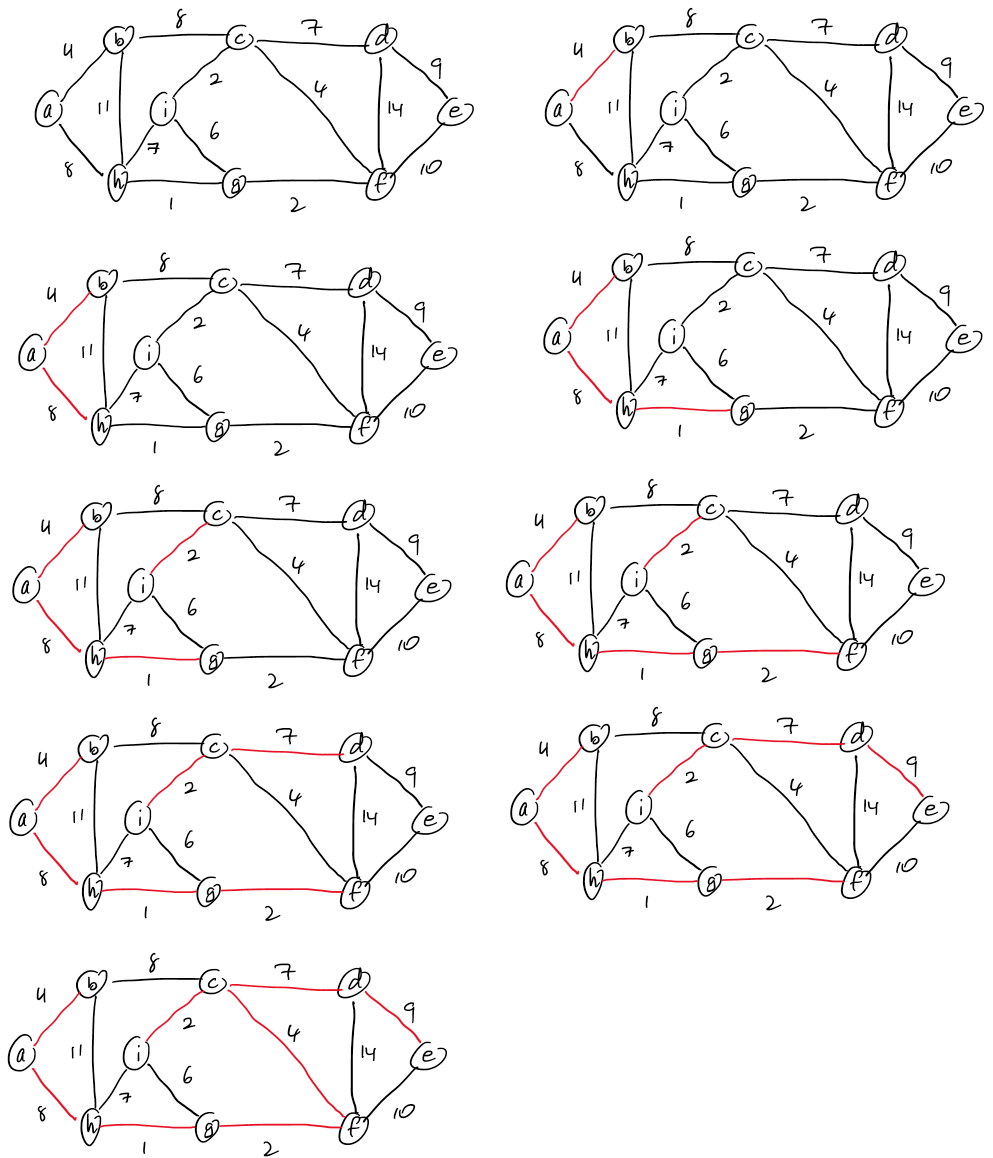
\includegraphics[scale=0.75]{Q9a}

\newpage

		\item Minimum spanning tree with Kruskal’s Algorithm: \\
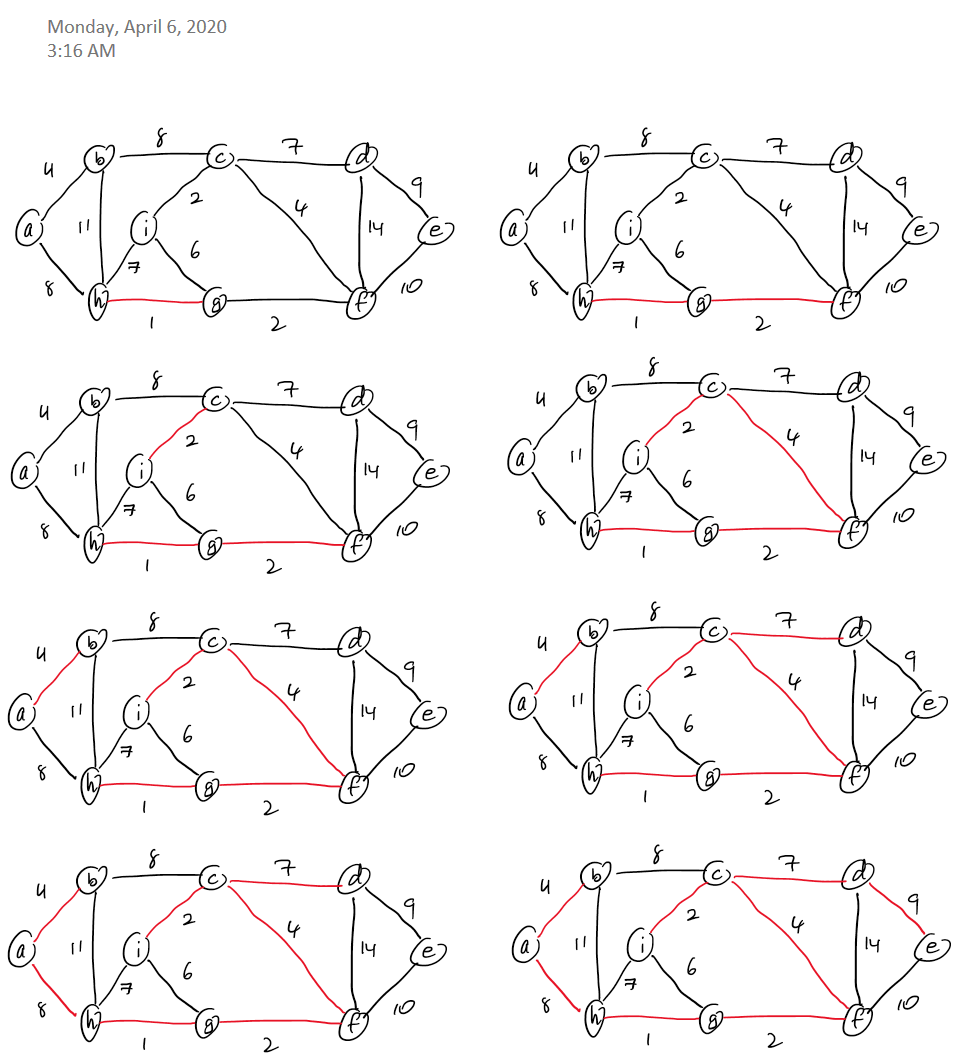
\includegraphics[scale=0.75]{Q9b}

\newpage

		\item Minimum spanning tree with Prim’s Algorithm: \\
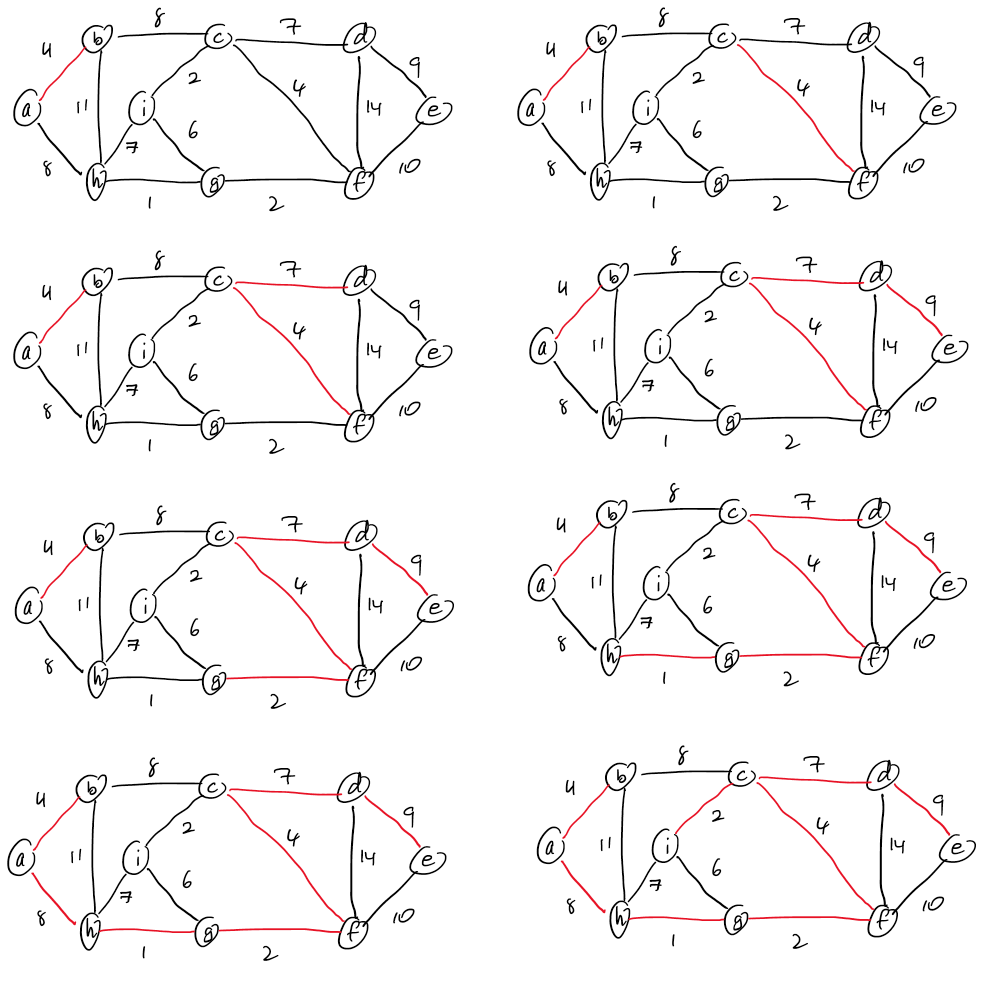
\includegraphics[scale=0.75]{Q9c}
	\end{enumerate}

%Q10
	\item
a to a (0.00)  \\
a to b (2.00)  a$\rightarrow$b  2.00   \\
a to c (6.00)  a$\rightarrow$j  4.00   j$\rightarrow$c  2.00   \\
a to d (6.00)  a$\rightarrow$b  2.00   b$\rightarrow$f  3.00   f$\rightarrow$d  1.00   \\
a to e (8.00)  a$\rightarrow$l  5.00   l$\rightarrow$e  3.00   \\
a to f (5.00)  a$\rightarrow$b  2.00   b$\rightarrow$f  3.00   \\
a to h (5.00)  a$\rightarrow$h  5.00   \\
a to i (5.00)  a$\rightarrow$j  4.00   j$\rightarrow$i  1.00   \\
a to j (4.00)  a$\rightarrow$j  4.00   \\
a to k (7.00)  a$\rightarrow$b  2.00   b$\rightarrow$f  3.00   f$\rightarrow$d  1.00   d$\rightarrow$k  1.00   \\
a to l (5.00)  a$\rightarrow$l  5.00

%Q11
	\item
s to s ( 0.00)  \\
s to t ( 2.00)  s$\rightarrow$y  7.00   y$\rightarrow$x -3.00   x$\rightarrow$t -2.00   \\
s to x ( 4.00)  s$\rightarrow$y  7.00   y$\rightarrow$x -3.00   \\
s to y ( 7.00)  s$\rightarrow$y  7.00   \\
s to z (-2.00)  s$\rightarrow$y  7.00   y$\rightarrow$x -3.00   x$\rightarrow$t -2.00   t$\rightarrow$z -4.00   \\

%Q12
	\item 
\begin{Verbatim}
public double diameter(EdgeWeightedDigraph edgeWeightedDigraph) {
	double diameter = Double.NEGATIVE_INFINITY;

	for (int v = 0; v < edgeWeightedDigraph.V(); v++) {
		DijkstraSP dijkstraSP = new DijkstraSP(edgeWeightedDigraph, v);

		for (int v2 = 0; v2 < edgeWeightedDigraph.V(); v2++) {
			if (dijkstraSP.distTo(v2) > diameter) {
				diameter = dijkstraSP.distTo(v2);
			}
		}
	}

	return diameter;
}
\end{Verbatim}

%Q13
	\item
r to r (0.00)  
r to s (5.00)  r->s  5.00   
r to t (3.00)  r->t  3.00   
r to x (10.00)  r->t  3.00   t->x  7.00   
r to y (7.00)  r->t  3.00   t->y  4.00   
r to z (5.00)  r->t  3.00   t->z  2.00

%Q14
	\item
	\begin{enumerate}
		\item
Give a trace for LSD string sort for the keys:  \\
no is th ti fo al go pe to co to th ai of th pa 
\begin{Verbatim}
input   d=1   d=0   output 
no      pa    ai    ai
is      pe    al    al
th      of    co    co
ti      th    fo    fo
fo      th    go    go
al      th    is    is
go      ti    no    no
pe      ai    of    of
to      al    pa    pa
co      no    pe    pe
to      fo    th    th
th      go    th    th
ai      to    th    th
of      co    ti    ti
th      to    to    to
pa      is    to    to
\end{Verbatim}

		\item
Give a trace for MSD string sort for the keys: \\
no is th ti fo al go pe to co to th ai of th pa
\begin{Verbatim}
input   --      --                      output
no      al      ai      ai      ai      ai       
is      ai      al      al      al      al
th      co      --      co      co      co
ti      fo      co      fo      fo      fo
fo      go      fo      go      go      go
al      is      go      is      is      is
go      no      is      no      no      no
pe      of      no      of      of      of
to      pe      of      --      pa      pa
co      pa      pe      pa      pe      pe
to      th      pa      pe      --      th
th      ti      th      --      th      th
ai      to      ti      th      th      th
of      to      to      ti      th      ti
th      th      to      to      ti      to
pa      th      th      to      to      to
        --      th      th      to
                        th      --
\end{Verbatim}

		\item
Give a trace for MSD string sort for the keys: \\
now is the time for all good people to come to the aid of
\begin{Verbatim}
input       ---        ---                                 output            
now         all         aid         aid         aid         aid         
is          aid         all         all         all         all
the         come        ---         come        come        come
time        for         come        for         for         for
for         good        for         good        good        good
all         is          good        is          is          is
good        now         is          now         now         now
people      of          now         of          of          of
to          people      of          people      people      people
come        the         people      ---         ---         the
to          time        the         the         the         the
the         to          time        the         the         time
aid         to          to          time        ---         to
of          the         to          to          time        to
            ----        the         to          to
                                    ---         to
\end{Verbatim}
	\end{enumerate}
	
%Q15
	\item $~$\\
%\includegraphics[scale=0.75]{Q15}

%Q16
	\item 
\begin{Verbatim}
Failure Function:
P = abbababaaabab
j     0 1 2 3 4 5 6 7 8 9 10 11 12
P[j]  a b b a b a b a a a b  a  b
f(j)  0 0 0 1 2 1 2 1 1 1 2  1  2



Solution using Knuth-Morris-Pratt algorithm:
abaababaababbababaaababaabaababb
123
abbababaaabab
  45
  abbababaaabab
   678
   abbababaaabab
-----------------------------
a b a a b a b a a b a b b a b a b a a a b a b a a b a a b a b b
                9 1011
                a b b a b a b a a a b a b
-----------------------------
a b a a b a b a a b a b b a b a b a a a b a b a a b a a b a b b
                    12131415161718192021222324
                    a b b a b a b a a a b a b

Final Answer:
abaababaababbababaaababaabaababb
          abbababaaabab
\end{Verbatim}
The algorithm performs 24 character comparisons, which are
indicated with numerical labels.

%Q17
	\item 

%Q18
	\item 

%Q19
	\item 

%Q20
	\item 

%Q21
	\item 

\end{enumerate}

\end{document}


